\documentclass[a4paper]{bxjsarticle}
\usepackage[oldxetex]{zxjatype}
\setjamainfont{IPA明朝}
\setjasansfont{IPAゴシック}
\setjamonofont{IPAゴシック}
\usepackage{xltxtra}
% 欧文は既定の LM フォント
\begin{document}
\title{{\XeLaTeX}で日本語する件について}
\author{ZR}
\date{2010年\ 某月\ 某日}
\maketitle

\section{{\XeTeX}\>の紹介}

\subsection{{\XeTeX}\>とは}

{\XeTeX}\>はJonathan Kew氏による\>{\TeX}\>の拡張で符号空間を
Unicode全体(BMP以外も含む)に拡大したものである。
既存の\>{\TeX}\>のUnicode拡張としてはOmega(Ω)
があるが、{\XeTeX}\>はこれとは別の拡張となっている。%
(なお、Omegaの後継にあたるUnicode拡張\>{\TeX}\>が\>%
{Lua\TeX}\>である。)

{\XeTeX}\>のもう一つの大きな特徴は、現在の標準的なフォント技術を
内部に取り込んでいることである。
元々の\>{\TeX}\>が「特定の技術基盤に依存しない」という思想で設計されている
ことはよく知られているが、これはフォント関係の技術についても当てはまり、
フォントの扱いは\>{\TeX}\>本体(すなわち\>{\TeX}\>ソースをDVI%
ファイルに変換する)ではなくDVIウェア(DVIファイルを扱う
ソフトウェア)が行う。
このため、{\TeX}\>の機能自体は30年前からほとんど変わっていないにも
関わらず、dvipdfmxと組み合わせてOpenTypeフォントを埋め込んだ%
PDF文書を作成するということが可能になっている。
しかしその代償として、例えば新しいフォントを使えるようにするために一定の作業が
必要になるなどの短所を持ち合わせている。
{\XeTeX}\>はこの点に関して「非依存性」を捨てて、システムで使用可能な
フォントを直接扱うことで、何も設定しなくても好きなフォントを使うことが可能に
なっている。
また、従来の\>{\TeX}\>では難しい、フォントのもつ情報を利用した高度なリガチャ・
アクセント付加・位置異形の処理も自由に使うことが可能になっている。

\subsection{{\XeTeX}\>の出力例}

{\XeTeX}\>のもつ能力の一端を示す例をあげる。
これは\>{\XeLaTeX}({\XeTeX}\>上で動く\>{\LaTeX})の文書である。

\jafamilyinverbatim % verbatim を和文フォントで出力
\begin{quote}\small\begin{verbatim}
% このファイルの文字コードは UTF-8
\documentclass[a4paper]{article}
\usepackage{xltxtra} % これは後で解説
\newfontfamily\fchr{Charis SIL}  % \fchr でフォント“Charis SIL”に切替
\newfontfamily\fipm{IPA明朝}     % \fipm でフォント“IPA明朝”に切替
  % \faru でデーヴァナーガリー文字用の設定を施した“Arial Unicode MS”に切替
\newfontfamily\faru[Script=Devanagari]{Arial Unicode MS}
  % \showUC は何の変哲のない LaTeX のマクロ
\newcommand*\showUC[1]{\ \texttt{\footnotesize U+#1}}
\begin{document}
\begin{itemize}
\item {\fipm 土\symbol{"571F}}\showUC{571F} /
      {\fipm 圡\symbol{"5721}}\showUC{5721} /
      {\fipm 𡈽\symbol{"2123D}}\showUC{2123D}
\item {\fchr j}\showUC{006A} + {\fchr\symbol{"0302}}\showUC{0302}
      = {\fchr j\symbol{"0302}}
\item {\fipm か}\showUC{304B} + {\fipm\symbol{"309A}}\showUC{309A}
      = {\fipm か\symbol{"309A}}
\item {\faru \symbol{"915}}\showUC{0915} + {\faru\symbol{"93F}}\showUC{093F}
      = {\faru \symbol{"915}\symbol{"93F}}
\end{itemize}

\end{document}
\end{verbatim}\end{quote}

上の文書をxelatexコマンドで組版すると以下の出力を含む%
PDF文書が得られる。

\begin{center}
\frame{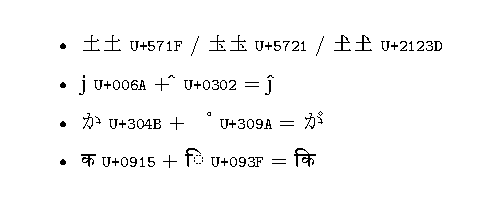
\includegraphics{xetexsamp01.pdf}}
\end{center}

\nojafamilyinverbatim % verbatim を欧文フォントで出力

上の文書において、\verb|\symbol{"xx}|\>は符号位置がxx(16進)である
文字を出力する\>{\LaTeX}\>コマンドである。
{\XeLaTeX}\>ではこれがUnicode符号空間で使えることが出力の
1行目から判る。%
(従来の\>{\LaTeX}\>では8ビットの値のみ。)
勿論、UTF-8で直接書いた文字も出力されている。
2行目以下ではUnicode結合文字を用いた文字合成の例を示している。%
\verb|j\symbol{"0302}|\>はjの直後にU+0302の文字
(結合曲アクセント)を書いたのと同じで、これはUnicodeの規則で
「ĵ(曲アクセント付j)」を表す。
2行目を見ると正しく合成が行われていることが判る。

\end{document}
